% *********************************************************************
% © 2016–2024 Jeremy Sylvestre
%
% Permission is granted to copy, distribute and/or modify this document
% under the terms of the GNU Free Documentation License, Version 1.3 or
% any later version published by the Free Software Foundation; with no
% Invariant Sections, no Front-Cover Texts, and no Back-Cover Texts. A
% copy of the license is included in the appendix entitled “GNU Free
% Documentation License” that appears in the output document of this
% PreTeXt source code. All trademarks™ are the registered® marks of
% their respective owners.
%
% *********************************************************************
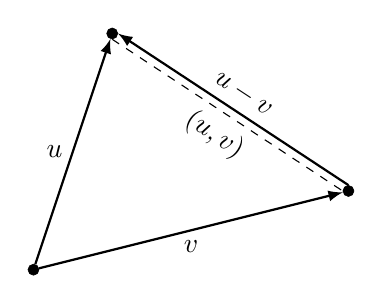
\begin{tikzpicture}[
	point/.style={circle,draw,very thin,fill,inner sep=0pt,minimum size=4pt},
	vector/.style={-latex},
]
	\node[point] at (0,0) (o) {};
	\node[point] at (1,3) (u) {};
	\node[point] at (4,1) (v) {};
	\draw[vector,thick] (o) to node[left] {$\uvec{u}$} (u);
	\draw[vector,thick] (o) to node[below] {$\uvec{v}$} (v);
	\draw[vector,thick] (v.north) to node[above,sloped] {$\uvec{u}-\uvec{v}$} (u.east);
	\draw[dashed] (u.south) to node[sloped,below] {$\dist(\uvec{u},\uvec{v})$} (v.west);
\end{tikzpicture}
